% Chapter 6

\chapter{Desenvolvimento} % Main chapter title
\label{chap:Chapter6} % For referencing the chapter elsewhere, use \ref{chap:Chapter6} 

	Neste capítulo são abordadas as principais decisões tomadas pelo autor durante a implementação das funcionalidades planeadas para o projeto. Para além das ferramentas e tecnologias utilizadas, é apresentada a metodologia seguida durante o desenvolvimento e a estrutura adotada para o \textit{backend}. São também descritas as principais integrações realizadas e as opções tomadas na utilização do \gls{LLM}, bem como algumas considerações relacionadas com os dados, custos e tempo de execução.

%----------------------------------------------------------------------------------------
\section{Stack Tecnológica}

	No início do projeto realizou-se uma análise sobre quais as melhores ferramentas e plataformas para o desenvolvimento do mesmo. Este capítulo apresenta as escolhas realizadas explicando os motivos de cada seleção.
	
%----------------------------------------------------------------------------------------
	\subsection{Python}
		A linguagem \textit{Python} foi escolhida para o desenvolvimento da solução principalmente pela sua forte utilização na área da Inteligência Artificial e pela variedade de bibliotecas disponíveis. Como o projeto envolve a utilização de \gls{LLM}s, processamento de texto e implementação de uma arquitetura \gls{RAG}, \textit{Python} permite integrar estas diferentes componentes de forma relativamente simples.
		
		Outro fator importante foi a facilidade de integração com serviços externos. A solução necessita de comunicar com o serviço de incidentes, com o motor \gls{LLM} e com os restantes componentes utilizados na recuperação de informação. \textit{Python} disponibiliza várias bibliotecas para comunicação através de \textit{APIs} e para trabalhar com diferentes formatos de dados, o que facilita esta integração.
		
		A linguagem também permite desenvolver e testar diferentes abordagens sem uma grande complexidade. Isto é particularmente importante neste projeto, uma vez que serão avaliadas diferentes configurações da solução, como a utilização de diferentes estratégias de recuperação e diferentes formas de fornecer contexto ao \gls{LLM}. A existência de bibliotecas para testes, processamento de dados e avaliação dos resultados facilita ainda o desenvolvimento da componente experimental do trabalho.
		
		Por fim, e ainda mais importante, \textit{Python} apresenta uma sintaxe simples e uma comunidade bastante ativa, o que facilita a implementação das diferentes funcionalidades. Tendo em conta estas características e as necessidades da solução, considerou-se que \textit{Python} seria uma escolha adequada para implementar o serviço e testar as diferentes abordagens propostas.
		
	%----------------------------------------------------------------------------------------
	\subsection{RAG}
		A utilização de \gls{RAG} foi escolhida para permitir que o \gls{LLM} tenha acesso ao histórico de incidentes no momento da análise, sem depender apenas do conhecimento que o modelo possui. Esta abordagem é particularmente adequada ao problema em estudo, uma vez que os incidentes estão constantemente a ser criados e atualizados. Desta forma, novos incidentes podem ser utilizados como contexto sem ser necessário voltar a treinar o modelo.
		
		Para a recuperação dos incidentes optou-se por uma abordagem baseada na informação já disponível no \textit{ServiceNow}, em vez da utilização de \textit{embeddings}. A \gls{API} do serviço externo permite obter a lista de incidentes da equipa e os respetivos dados, sendo possível aplicar filtros e, posteriormente, ordenar os resultados pelos incidentes mais recentes. Esta abordagem é suficiente para o contexto deste projeto, uma vez que grande parte dos incidentes analisados (98.41\%) é gerada automaticamente pelos sistemas de monitorização e segue padrões semelhantes. Nestes casos, a utilização de uma pesquisa semântica através de \textit{embeddings} não apresenta uma vantagem clara face à utilização dos dados estruturados já disponíveis.
		
		Esta opção permite também manter o processo de recuperação mais simples e fácil de controlar. Em vez de criar e manter uma base de dados de \textit{embeddings}, os incidentes são obtidos diretamente da fonte de informação existente e filtrados de acordo com as necessidades da análise. Os incidentes selecionados são depois utilizados como contexto para o \gls{LLM}, que fica responsável por analisar a informação e gerar a resposta.
		
		A escolha de \gls{RAG} em vez de \textit{fine-tuning} está também relacionada com a natureza dos dados. O \textit{fine-tuning} permite adaptar o comportamento do modelo a uma determinada tarefa, mas não é a melhor opção quando o objetivo principal é fornecer informação que está constantemente a mudar. No caso dos incidentes, novos comentários e as respetivas resoluções surgem regularmente, o que obrigaria a atualizar o treino do modelo para acompanhar a informação mais recente. Com \gls{RAG}, essa informação pode ser obtida diretamente da fonte de dados e utilizada pelo modelo durante cada análise, sem necessidade de novo treino.
		
		Assim, a abordagem escolhida procura aproveitar a informação histórica já disponível no \textit{ServiceNow}, mantendo o processo de recuperação simples e permitindo que o \gls{LLM} tenha acesso a informação atualizada. O \textit{fine-tuning} poderia ser utilizado como complemento no futuro, caso fosse necessário adaptar o comportamento ou o formato das respostas do modelo.
	
	%----------------------------------------------------------------------------------------
	\subsection{Langfuse}
		Para acompanhar a utilização dos \gls{LLM}s foi utilizado o \textit{Langfuse}, permitindo obter uma maior visibilidade sobre as operações realizadas durante cada pedido. A ferramenta permite acompanhar as diferentes chamadas ao modelo e os respetivos custos, tornando possível perceber quanto é gasto em cada etapa do processo de análise de um incidente.
		
		Esta informação é importante para a avaliação da solução, uma vez que permite calcular o custo associado a cada pedido e identificar quais as operações que têm maior impacto no consumo. Desta forma, é possível não só acompanhar os custos da solução, mas também identificar oportunidades de otimização.
		
		A utilização do \textit{Langfuse} permite ainda que esta análise possa ser expandida no futuro. Para além do custo por pedido, poderão ser analisadas outras dimensões, como os custos associados a diferentes utilizadores, sessões ou tipos de operação. Isto permite obter uma visão mais detalhada sobre a utilização do sistema e apoiar futuras decisões de otimização.

%----------------------------------------------------------------------------------------
\section{Metodologia de Implementação}
	
	Nesta secção é demonstrada a metodologia escolhida para o desenvolvimento do projeto (\gls{SDD}), assim como as razões que motivam essa escolha, as limitações, os métodos utilizados para combater os problemas causados pela metadologia e a forma como foi implementada.
	
%----------------------------------------------------------------------------------------
	\subsection{Spec Driven Development}
	
		O desenvolvimento de software tem sido baseado em diferentes formas de organizar e controlar o processo de implementação. Com o aumento da complexidade dos sistemas e, mais recentemente, com a utilização de ferramentas de \gls{IA} na programação, tornou-se cada vez mais importante definir de forma clara aquilo que se pretende desenvolver antes de iniciar a implementação. Quando o desenvolvimento começa diretamente pelo código, surgem, normalmente, problemas relacionados com requisitos pouco claros, decisões técnicas inconsistentes e diferenças entre o comportamento esperado e o comportamento implementado.
		
		Esta metodologia coloca as especificações no centro do processo de desenvolvimento, sendo utilizadas como referência para definir e implementar as diferentes funcionalidades do sistema. Ao invés de começar diretamente pela implementação, cada funcionalidade é primeiro descrita e detalhada através de uma especificação. A partir dessa documentação é definido o plano de implementação e, de seguida, as tarefas necessárias para desenvolver a funcionalidade.
		
		Esta abordagem foi escolhida principalmente devido à utilização de \gls{IA} como apoio ao desenvolvimento. Ao definir primeiro aquilo que o sistema deve fazer, é possível fornecer ao agente uma descrição mais clara do objetivo e das condições que a implementação deve cumprir. Desta forma, a utilização de \gls{IA} não fica limitada à geração direta de código a partir de um pedido, mas é incluída num processo mais estruturado.
	
		Apesar da existência de um kit oficial de ferramentas (\textit{spec-kit}), optou-se por aplicar \gls{SDD} diretamente assim, a aplicação da metodologia, não ficou dependente da estrutura definida pela ferramenta. Por esse motivo, o projeto conta com uma série de ficheiros documentais que ajudam tanto no processo de criação de especificações, como também no processo de implementação.
		
		A utilização desta abordagem permitiu ainda dedicar mais tempo ao pensamento crítico e à compreensão do negócio, em vez de focar principalmente na implementação do código. Desta forma, foi possível dar maior atenção às decisões e ao problema que a solução pretendia resolver.
	
%----------------------------------------------------------------------------------------
	\subsection{Limitações}
		
		Apesar das vantagens desta abordagem, identificaram-se algumas limitações durante o desenvolvimento. Uma delas foi o \textit{spec drift}, que ocorre quando são realizadas alterações no código sem que a respetiva especificação seja atualizada de forma prévia. Por exemplo, uma alteração feita através de \textit{vibe coding}, como adicionar uma lógica de \textit{retry} ao pedido feito ao \textit{ServiceNow}, pode ser implementada diretamente sem passar pelo processo definido pelo \gls{SDD}. Assim, o agente só segue esta abordagem quando essa disciplina é imposta pelo utilizador, podendo uma instrução simples levar à implementação direta e deixar a especificação desatualizada.
		
		Outra limitação está relacionada com o esforço adicional (\textit{overhead}) associado a pequenas alterações. Mesmo uma alteração simples pode exigir a atualização da especificação, a implementação e a posterior validação. Embora este processo ajude a manter o código alinhado com as especificações, pode representar um esforço adicional para alterações de pequena dimensão.
	
%----------------------------------------------------------------------------------------
	\subsection{Agentic \gls{SDD}}
	
		Com objetivo de apoiar o desenvolvimento e ajudar a garantir o cumprimento do processo definido pelo \gls{SDD} foram criados agentes. Um agente pode ser visto como um assistente que, para além de responder a instruções, consegue seguir um conjunto de regras, consultar informação disponível no projeto e realizar diferentes tarefas de acordo com o contexto fornecido. Para além de ajudarem na criação e atualização das \textit{specs}, os agentes são instruídos a consultar informação adicional do projeto antes de realizar alterações. Esta informação encontra-se organizada em diferentes ficheiros, nomeadamente:
		
		\begin{itemize}
			\item \textbf{\textit{Template} para as especificações} - Modelo base de uma especificação. Define os capítulos que todas as especificações devem conter assim como tópicos que devem ser abordados dentro de cada secção;
			\item \textbf{Arquitetura} - Descreve a arquitetura pretendida para o projeto. Define quais as camadas e como devem ser organizadas;
			\item \textbf{Requisitos} - Define os requisitos funcionais, não funcionais e de observabilidade do sistema;
			\item \textbf{Especificação da API} - Descreve as especificações da API a ser desenvolvida, definindo os parâmetros de entrada e saída do serviço.
		\end{itemize}
		
		Estes documentos foram o passo zero da implementação do projeto, servindo de base para iniciar a descrição as funcionalidades, objetivos pretendidos e a forma de os alcançar.
		Após essa definição foram criados os agentes que permitiriam aplicar o processo SDD ao desenvolvimento do projeto. Assim, os agentes criados foram:
		
		\begin{itemize}
			\item \textbf{Arquiteto de especificações} - Interpreta o contexto fornecido pelo desenvolvedor, define critérios de aceitação, cria/atualiza especificações de acordo com o modelo definido e atualiza outros documentos quando necessário. Nunca implementa código nem testes;
			\item \textbf{Engenheiro de \textit{Software}} - Interpreta as especificações já criadas, cria tarefas orientadores, implementa código e testes e valida as implementações realizadas. Nunca altera especificações, quando deteta essa necessidade deve invocar o agente responsável;
			\item \textbf{Agente de validação} - Compara implementações com especificações, valida a cobertura de critérios de aceitação e pede correções quando necessário.
		\end{itemize}
		
		A utilização destes agentes, permite não só automatizar parte das tarefas associadas ao \gls{SDD}, mas também orientar o desenvolvedor durante todo o processo garantindo que o contexto necessário é considerado antes da implementação.
	
%----------------------------------------------------------------------------------------
	\subsection{Specs}
		
		As especificações foram organizadas em ficheiros próprios dentro da pasta \texttt{docs/specs/}, seguindo o modelo definido no início do projeto, como demonstrado na figura \ref{fig:specTemplate}. Este modelo permite manter uma estrutura semelhante entre as diferentes especificações e facilita a sua consulta e atualização ao longo do desenvolvimento.
		
		\begin{figure}[H]
			\centering
			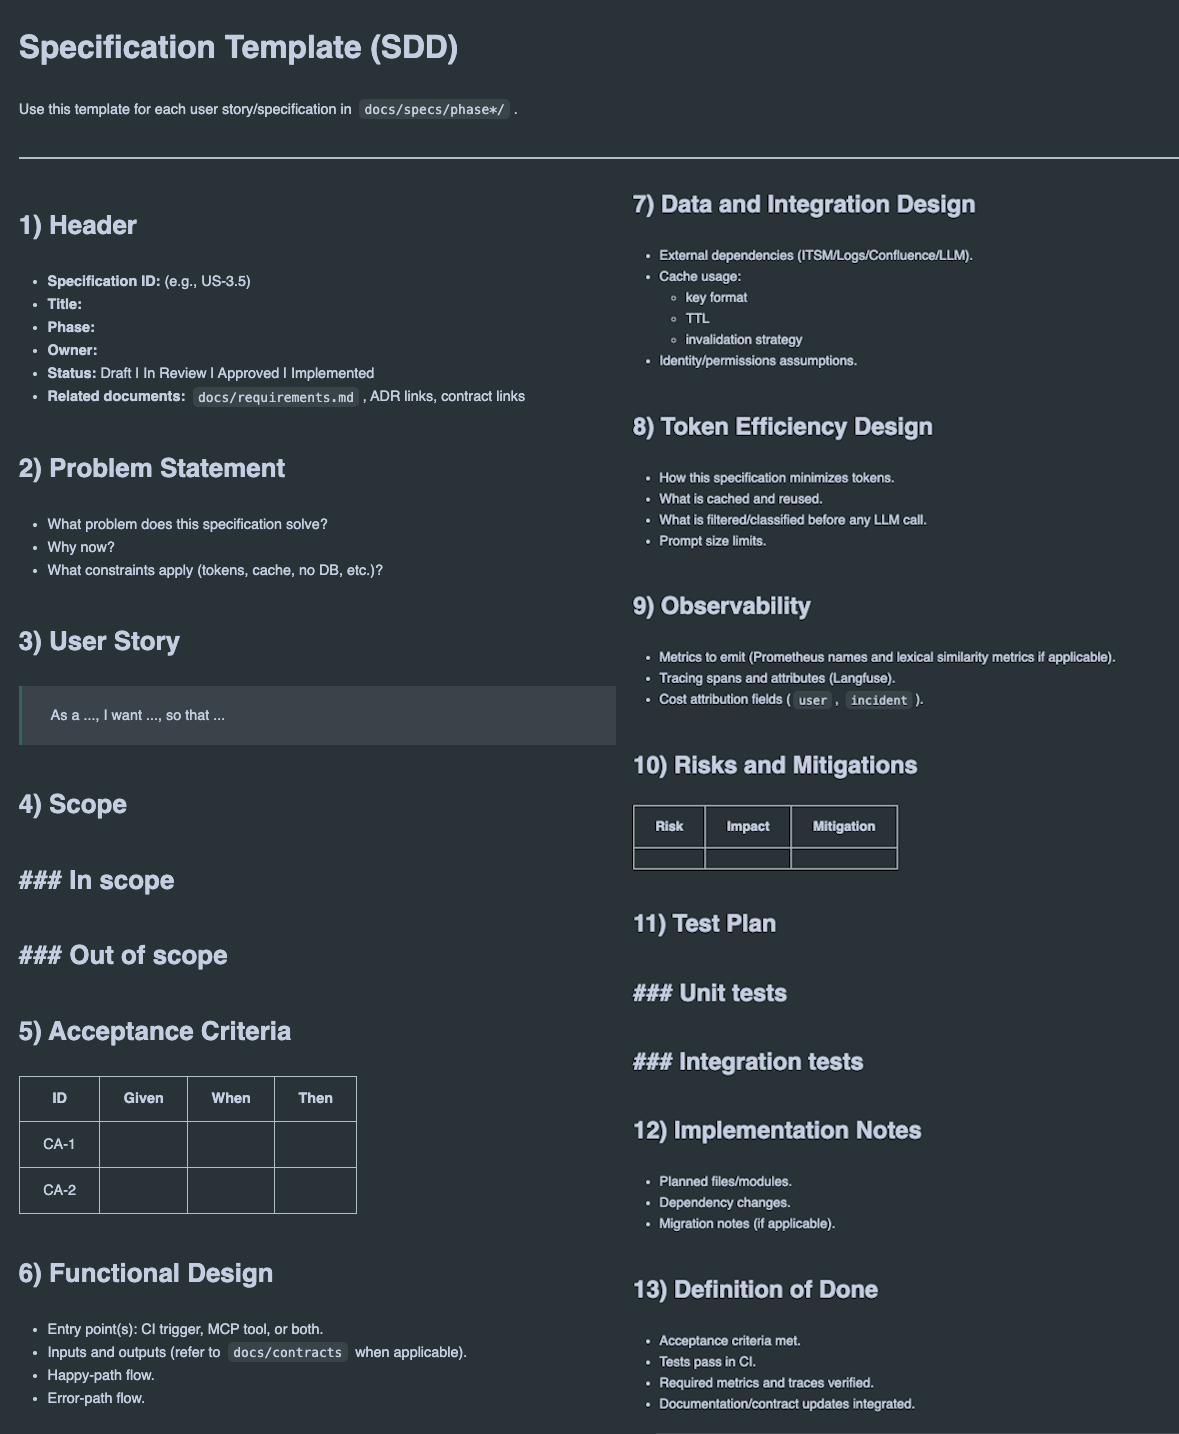
\includegraphics[width=130mm,keepaspectratio]{img/spec_template}
			\caption[Modelo Base de uma Especificação]{Modelo Base de uma Especificação}
			\label{fig:specTemplate}
		\end{figure}
		
		Cada especificação contém a informação necessária para orientar o desenvolvimento da funcionalidade, incluindo o problema a resolver, os objetivos, os critérios de aceitação, as integrações com serviços externos, o plano de testes e as alterações necessárias. A especificação pode ser atualizada ao longo do desenvolvimento sempre que sejam identificadas novas necessidades ou alterações ao comportamento esperado.
		
		Todo este trabalho deve ser realizado com o uso do Arquiteto de especificações para que, no momento da criação das espeficificações, o agente saiba que documentos extra deve ter em conta para além do contexto dado pelo desenvolvedor. 
		
		Já o desenvolvimento foi dividido em diferentes fases, permitindo adicionar funcionalidades de forma gradual e validar cada etapa antes de avançar para a seguinte. A primeira fase esteve focada na criação da \textit{API} e na primeira integração com o \gls{LLM}. A segunda fase adicionou contexto de incidentes, observabilidade e integração com a documentação do \textit{Confluence}. Por fim, a terceira fase contém uma funcionalidade que já foi especificada e preparada para implementação, mas que ficou fora do âmbito do trabalho desenvolvido.
		
		A seguinte lista apresenta as especificações criadas ao longo do desenvolvimento, agrupadas por fase:
		
		\begin{itemize}
			\item \textbf{Fase 1}
			\begin{itemize}
				\item \textit{US-1.1: Disponibilização da \gls{API} de detalhes do incidente}
				\item \textit{US-1.2: Obtenção dos dados base do incidente a partir do cliente}
				\item \textit{US-1.3: Integração do enriquecimento com \gls{LLM} no \textit{GET} \texttt{/incident/details}}
				\item \textit{US-1.4: Registo do custo de utilização do \gls{LLM} e do tempo de resposta}
				\item \textit{US-1.5: Avaliação manual entre versões}
			\end{itemize}
			
			\item \textbf{Fase 2}
			\begin{itemize}
				\item \textit{US-2.1: Adição da análise de logs e de observabilidade mais detalhada}
				\item \textit{US-2.2: Implementação de rastreabilidade distribuída com \textit{Langfuse} e \textit{OpenTelemetry}}
				\item \textit{US-2.3: Integração do contexto de incidentes relacionados no enriquecimento com \gls{LLM}}
				\item \textit{US-2.4: Pesquisa alternativa por incidentes recentes da equipa quando não são encontrados incidentes com o mesmo título}
				\item \textit{US-2.5: Utilização de um \gls{LLM} para encontrar incidentes relacionados e documentação do serviço no Confluence}
			\end{itemize}
			
			\item \textbf{Fase 3}
			\begin{itemize}
				\item \textit{US-3.1: Integração da base de dados de \textit{logs} para fornecer registos de transações relacionados como contexto para o \gls{LLM}}
			\end{itemize}
		\end{itemize}
		
		A organização das especificações por fases permitiu acompanhar a evolução da solução e manter o desenvolvimento dividido em partes mais pequenas. Desta forma, cada nova funcionalidade podia ser analisada, implementada e validada antes de avançar para a fase seguinte.

%----------------------------------------------------------------------------------------
\section{Estrutura}

	A arquitetura do projeto definiu-se com base em princípios de \gls{DDD}, adaptados às necessidades de um protótipo de apoio à análise de incidentes. O objetivo foi manter a lógica relacionada com o negócio separada das tecnologias e serviços externos utilizados pelo sistema.
	
	O domínio do projeto está centrado na análise e correlação de incidentes, incluindo a interpretação da informação dos \textit{tickets}, a identificação de incidentes relacionados, a organização da informação e a geração de sugestões de mitigação. Desta forma, a lógica principal do serviço não fica diretamente dependente das \gls{API}\textit{s} ou tecnologias utilizadas para obter ou processar esta informação.
	
	Para garantir esta separação, o projeto foi dividido em três camadas principais, como demonstra a figura \ref{fig:projectStructure}. A camada \textit{domain} contém os modelos e regras de negócio, bem como as interfaces necessárias para comunicar com serviços externos. A camada \textit{infrastructure} contém as implementações dessas interfaces e é responsável pela comunicação com sistemas como o \gls{ITSM} e os serviços de \gls{LLM}. Por fim, a camada \textit{presentation} é responsável pela exposição da aplicação, nomeadamente através da \textit{API REST}.
	
	\begin{figure}[H]
		\centering
		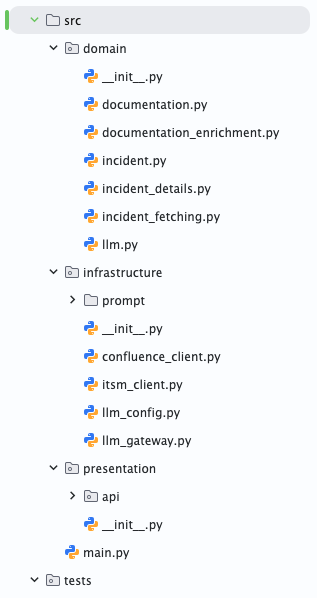
\includegraphics[width=60mm,keepaspectratio]{img/project_structure_v2}
		\caption[Estrutura do Protótipo]{Estrutura do Protótipo}
		\label{fig:projectStructure}
	\end{figure}
	
	Esta organização foi escolhida para dar resposta ao \textit{RNF-02}, que define que o sistema deve permitir adicionar, substituir ou remover serviços externos sem impacto no restante serviço. Ao manter as integrações externas isoladas na camada de infraestrutura e ao definir os seus contratos no domínio, é possível substituir uma implementação sem alterar diretamente a lógica de negócio. Por exemplo, a integração com um determinado fornecedor de \textit{LLM} pode ser substituída por outra implementação sem necessidade de alterar as regras utilizadas na análise dos incidentes.
	
	Assim, a estrutura adotada permite manter o núcleo da aplicação independente das tecnologias externas, facilitando futuras alterações e reduzindo o impacto das mudanças nas integrações. Simultaneamente, mantém uma organização simples e adequada ao âmbito do projeto, evitando uma separação excessivamente complexa para as necessidades do protótipo.
	
%----------------------------------------------------------------------------------------
\section{Implementação}

	A aplicação integra diferentes fontes de informação e serviços externos, sendo necessário tratar e organizar essa informação antes de a disponibilizar ao \gls{LLM}. 
	
	A implementação é apresentada de acordo com os principais componentes envolvidos no processo. Primeiro, é descrita a integração com o sistema \gls{ITSM}, responsável pela obtenção do incidente principal e de informação sobre incidentes anteriores. De seguida, é apresentada a integração com o \textit{Confluence}, utilizada para obter documentação adicional relacionada com o problema. Posteriormente, é explicada a integração com o \gls{LLM}, incluindo a utilização dos diferentes \textit{prompts}, a análise da informação recolhida e a geração das sugestões de mitigação. Por fim, são apresentadas algumas decisões tomadas durante a implementação, nomeadamente a utilização de \gls{RAG}, o tratamento de dados sensíveis e o controlo dos custos e do tempo de execução.
	
%----------------------------------------------------------------------------------------
	\subsection{Integração com ITSM}
		
		A integração com o \gls{ITSM} (produto do \textit{ServiceNow}) foi responsável por obter a informação necessária para a análise do incidente principal e por disponibilizar a informação de incidentes anteriores para que fosse utilizada de seguida pelo \gls{LLM}. O processo foi dividido entre a obtenção do incidente principal e a recuperação de possíveis incidentes relacionados.
		
		%\subsubsection{Obtenção do Incidente Principal}
		
		O processo começa com a obtenção do incidente a ser analisado. A informação devolvida pelo \gls{ITSM} é, então, convertida para os modelos utilizados pelo domínio, permitindo que a restante aplicação trabalhe com uma estrutura independente da representação utilizada pelo sistema externo.
		
		São selecionados apenas os campos necessários para a análise do incidente e para fornecer contexto adicional ao \gls{LLM}. Desta forma, evita-se também a propagação de informação que não seja relevante ou que tenha sido identificada como sensível.
		
		% \subsubsection{Recuperação de Incidentes Relacionados}
		
		Após a obtenção do incidente principal, são realizadas pesquisas no \gls{ITSM} para obter possíveis incidentes relacionados. Nesta fase, o objetivo não é determinar se os incidentes estão efetivamente relacionados, mas sim recolher um conjunto de incidentes que possa posteriormente ser analisado pelo \gls{LLM}. São consideradas as referências no incidente principal através dos campos:
		
		\begin{itemize}
			\item \texttt{parent\_incident}
			\item \texttt{description}
			\item \texttt{close\_notes}
			\item \texttt{comments}
			\item \texttt{work\_notes}
			\item \texttt{hold\_reason}
		\end{itemize}
		
		Os incidentes encontrados são identificados pelo seu número, permitindo evitar duplicados durante o processo.
		
		A pesquisa é feita apenas a partir do incidente principal. Os incidentes obtidos nesta fase não são utilizados para procurar novos incidentes relacionados. Esta decisão evita que a pesquisa se torne recursiva e que sejam obtidos incidentes cada vez mais afastados do contexto do problema original.
		
		É ainda realizada uma pesquisa por incidentes que tenham o mesmo \texttt{short\_description} do incidente principal. Esta pesquisa permite encontrar ocorrências anteriores com um título semelhante, que podem conter informação útil sobre problemas e resoluções anteriores.
		
		%\subsubsection{Recuperação do Histórico de Incidentes}
		
		Quando a pesquisa por incidentes com o mesmo \texttt{short\_description} não produz resultados, é utilizado um mecanismo de \textit{fallback}. Neste caso, são obtidos incidentes mais recentes associados à equipa responsável, incluindo incidentes ativos e fechados. O objetivo deste mecanismo é garantir que o \gls{LLM} recebe algum contexto histórico mesmo quando não existem incidentes anteriores com o mesmo título. Este \textit{fallback} também permite ao \gls{LLM} ter em conta falhas no serviço que possam estar relacionados ou mesmo ser a causa de outro incidente.
			
			
	\subsection{Integração com Confluence}
		
		% Obtençao das páginas relacionadas
			% Explicar que a pesquisa não é feita em todo o Confluence, mas limitada ao espaço definido.
			% Nesta pesquisa percorre páginas e respetivas subpáginas
		% Obtenção do conteúdo da Documentação
		% Seleção da Informação Relevante (com ajuda do LLM mas não explorar muito isto e deixar para a integração com o LLM)
		% Integração da Documentação no Contexto
		
		O \textit{Confluence} é utilizado como uma fonte adicional de informação para complementar os dados obtidos através do \gls{ITSM}. O objetivo é encontrar documentação que possa ajudar a compreender melhor o problema identificado no incidente e que possa ser utilizada pelo \gls{LLM} durante a análise final.
		
		A pesquisa no \textit{Confluence} não é realizada sobre todas as páginas disponíveis. Para limitar os resultados da informação relevante para o projeto, a pesquisa é restringida ao espaço referente desse produto. A partir da informação do incidente são procuradas páginas que possam estar relacionadas com o projeto.
		
		Aquando da identificação das páginas relacionadas, é também obtido o seu conteúdo para que possa ser utilizado nas etapas seguintes. Posteriormente, o serviço recolhe as informações necessárias para identificar cada página, e permitir à aplicação conseguir manter a referência à origem da informação que será posteriormente utilizada no contexto enviado ao \gls{LLM}.
		
		A pesquisa pode devolver páginas que, apesar de estarem relacionadas com o projeto ou com os termos utilizados na pesquisa, não sejam relevantes para o incidente em análise. Por esse motivo, a informação obtida do \textit{Confluence} é analisada com o apoio do \gls{LLM}, que determina quais as páginas que apresentam informação útil para o problema atual e as resume como um "Homem das Cavernas" deixando apenas palavras chave.
		
		Após a seleção e resumo das páginas relevantes, o seu conteúdo é integrado com a restante informação recolhida durante o processo. Assim, o contexto final utilizado pelo \gls{LLM} pode incluir a informação do incidente principal, os incidentes relacionados e a documentação relevante do \textit{Confluence}. Para além do conteúdo, é mantida a referência para cada página selecionada, permitindo identificar posteriormente a documentação utilizada e apresentar ao utilizador a respetiva página como fonte de informação.
	
%----------------------------------------------------------------------------------------
	\subsection{Integração com LLM}
		% Explicar o que é LLM
		% Explicar como usamos LLM ( e introduzir o uso de prompts)
			%Explicar que foi divido em 3 chamadas em vez de uma grande
		% Explicar o que é prompt engineering
	
		% Prompt para obter incidentes relacionados e projeto afetado
		% Prompt para identificar documentação relevante ao problema
		% Preparação do Prompt da chamada final
			% Evolução do Prompt
			% Falar que a equipa escolheu comunicação simples, formal e human-readable (alguns escolheram mas ainda vou ter que falar com mais portnato ainda a confirma)
		
		% Estrutura da Informação Enviada
		% Geração das Sugestões de Mitigação
		% Conexão com o Langfuse
		
		Os \gls{LLM} são modelos de inteligência artificial treinados com grandes quantidades de dados textuais, sendo capazes de compreender e gerar texto em linguagem natural. Neste contexto, o \gls{LLM} foi utilizado para analisar a informação recolhida dos diferentes sistemas e transformá-la em conhecimento útil para a análise do incidente. Em vez de utilizar o modelo apenas para gerar uma resposta a partir do incidente principal, a aplicação utilizou-o em diferentes momentos do processo, permitindo realizar tarefas específicas antes de devolver a resposta final.
		
		A utilização do \gls{LLM} foi dividida em três fases de chamadas distintas. Esta divisão foi feita para evitar concentrar toda a informação e todas as tarefas numa única chamada, o que resultaria num \textit{prompt} maior e mais difícil de controlar. Na primeira fase, o modelo analisa o incidente principal e a informação dos incidentes candidatos obtidos através do \gls{ITSM}, identificando quais apresentam uma relação relevante com o problema atual e qual o projeto ou componente afetado. Desta forma, a aplicação não assume que todos os incidentes obtidos durante a pesquisa são realmente relacionados, deixando essa decisão para o modelo. De seguida, o \gls{LLM} analisa a documentação obtida através do \textit{Confluence} e determina quais as páginas que contêm informação relevante para o incidente. Nesta etapa, existem tantas chamadas quantas páginas forem retornadas pelo \textit{confluence}. Ao realizar chamadas individuais para cada página de documentação, evitamos criar um \textit{prompt} gigante, que poderia levar a alucinações e respostas incorretas por parte do modelo. A terceira e última fase, corresponde à análise final onde, são combinadas as informações selecionadas nas etapas anteriores para produzir as sugestões de mitigação.
		
		Para controlar o comportamento do modelo nestas diferentes fases, foram utilizados \textit{prompts} específicos. Um \textit{prompt} corresponde à informação e às instruções fornecidas ao \gls{LLM} para indicar o que deve ser analisado e qual o resultado esperado. A definição e melhoria destes \textit{prompts} enquadra-se no conceito de \textit{Prompt Engineering}, que consiste na criação e ajuste das instruções fornecidas ao modelo de forma a obter respostas mais consistentes e adequadas ao objetivo pretendido. Neste projeto, os \textit{prompts} foram sendo ajustados ao longo do desenvolvimento, tendo em consideração não só a informação disponível, mas também a forma como os resultados deveriam ser apresentados e utilizados pelas etapas seguintes.
		
		O primeiro \textit{prompt} é responsável pela análise dos incidentes candidatos. O modelo recebe a informação dos campos não sensíveis do incidente principal, sendo instruído a identificar, nesses campos, incidentes relacionados com o problema atual. Nesta mesma etapa é também identificado o projeto ou componente afetado, informação que será utilizada posteriormente para orientar a análise e apresentar sugestões. A pesquisa de incidentes é feita apenas a partir do incidente principal, não sendo realizada uma nova pesquisa com base nos incidentes identificados como relacionados. Esta decisão evita uma expansão sucessiva da pesquisa, na qual um incidente poderia levar à obtenção de outros incidentes apenas por estarem relacionados entre si, aumentando a quantidade de informação enviada ao modelo e o risco de incluir informação pouco relevante.
		
		O segundo \textit{prompt} é utilizado para analisar a documentação obtida através do \textit{Confluence}. A pesquisa inicial pode devolver páginas que estejam relacionadas com os termos utilizados, mas que não contenham informação útil para o problema específico. O \gls{LLM} recebe, por isso, o conteúdo das páginas encontradas e seleciona aquelas que apresentam informação relevante para o incidente. Para além de selecionar as páginas relevantes ao incidente, o modelo sumariza também as que considera relevantes, aplicando a técnica de sumarização \textit{caveman} onde se elimina palavras extra deixando apenas as palavras chave. O objetivo desta etapa não é gerar uma resposta final, mas reduzir a documentação disponível à informação que poderá contribuir para a análise seguinte.
		
		A última chamada recebe a informação selecionada nas etapas anteriores, incluindo os dados do incidente principal, os incidentes identificados como relacionados e a documentação considerada relevante. A preparação deste \textit{prompt} foi uma das partes que sofreu mais alterações durante o desenvolvimento, uma vez que pequenas alterações na forma de apresentar a informação ou nas instruções dadas ao modelo podiam influenciar o resultado obtido. O objetivo foi chegar a um formato que permitisse ao \gls{LLM} compreender facilmente o contexto e, ao mesmo tempo, produzir uma resposta que pudesse ser utilizada diretamente pela equipa de suporte. 
		
		A informação enviada ao \gls{LLM} é organizada de forma estruturada, separando os diferentes elementos que fazem parte do contexto. O incidente principal é apresentado como o problema que está a ser analisado, enquanto os incidentes relacionados e a documentação do \textit{Confluence} funcionam como informação adicional para ajudar na análise. Esta separação permite ao modelo distinguir a situação atual do histórico e da documentação utilizada como apoio. A aplicação também limita a quantidade de informação enviada ao modelo, evitando incluir dados que não sejam necessários para a análise e contribuindo para manter o custo e o tempo de execução dentro dos valores definidos para o sistema.
		
		Com base neste contexto, a chamada final gera sugestões de mitigação para o incidente. As sugestões são construídas tendo em consideração não só o incidente atual, mas também as soluções registadas em incidentes anteriores e a informação existente na documentação selecionada. Desta forma, o objetivo não é simplesmente solicitar ao \gls{LLM} que proponha uma solução genérica, mas fornecer-lhe informação relacionada com situações que já ocorreram e com o funcionamento do projeto afetado. A resposta produzida pelo modelo pode assim apresentar ações de mitigação que sirvam de apoio à equipa durante a resolução do incidente.
		
		Por fim, a integração com o \gls{LLM} é acompanhada através do \textit{Langfuse}. Esta ferramenta permite registar e acompanhar as diferentes chamadas realizadas durante uma análise, incluindo informação sobre o tempo de execução e os custos associados a cada pedido. Como o processo utiliza várias chamadas ao \gls{LLM}, esta observabilidade permite analisar cada operação individualmente e perceber quais as etapas que apresentam maior custo ou tempo de execução, como é visível na figura \ref{fig:langfuse_overall} e \ref{fig:langfuse_specific}. Estes dados podem também ser utilizados posteriormente para avaliar o comportamento do sistema e identificar possíveis oportunidades de otimização.
		
		\begin{figure}[H]
			\centering
			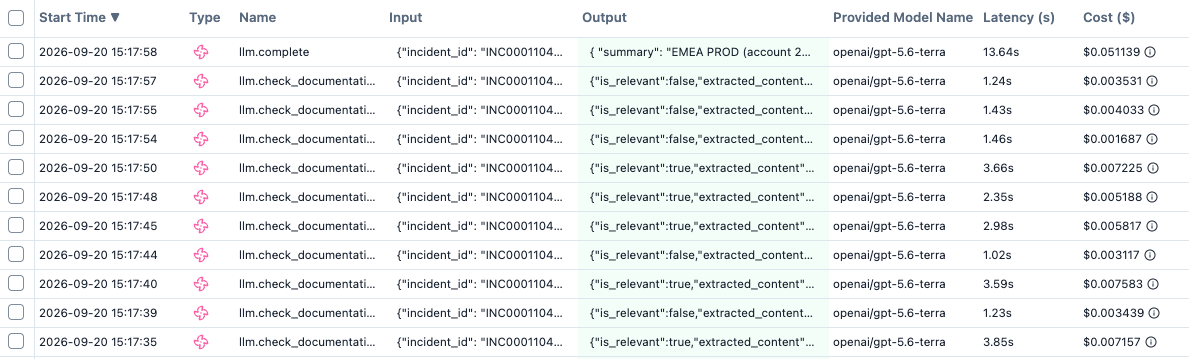
\includegraphics[width=\textwidth,keepaspectratio]{img/langfuse_overall}
			\caption[Exemplo de Registos no Langfuse]{Exemplo de Registos no Langfuse}
			\label{fig:langfuse_overall}
		\end{figure}
		
		\begin{figure}[H]
			\centering
			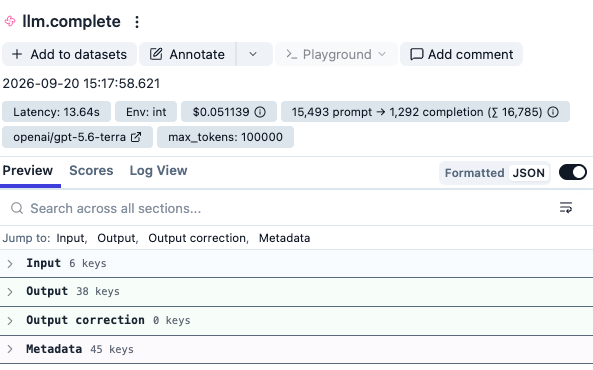
\includegraphics[width=100mm,keepaspectratio]{img/langfuse_specific}
			\caption[Exemplo de um Registo no Langfuse]{Exemplo de um Registo no Langfuse}
			\label{fig:langfuse_specific}
		\end{figure}
		
%----------------------------------------------------------------------------------------
	\subsection{Considerações de Implementação}
	
		\subsubsection{RAG vs Fine Tuning}
			% Explicar o que é RAG
			% Explicar o que é Fine Tuning
			
			% Explicar como usamos o RAG (tanto nos incidentes como na documentação)
			
			% Explicar porque não vetorizamos o RAG (sendo o contexto tão dinamico (em temos de mitigações) e ao mesmo tempo por maioria dos incidentes ser de cariz automática)
			
			Para o projeto foi escolhida a utilização de \gls{RAG}, devido sua à natureza dinâmica da informação usada durante a análise. Os incidentes existentes no \gls{ITSM} estão constantemente a ser alterados com a entrada de novos registos e, em particular, as informações relacionadas com a resolução dos incidentes podem mudar ao longo do tempo. O mesmo acontece com a documentação disponível no \textit{Confluence}. Com o uso de \gls{RAG}, esta informação pode ser obtida no momento da análise e fornecida ao modelo como contexto, sem ser necessário alterar o modelo sempre que são adicionados novos dados. No caso do \textit{Fine Tuning}, os novos dados teriam de ser novamente utilizados num processo de treino para que fossem incorporados pelo modelo.
			
			Para o caso dos incidentes, são recuperados do \gls{ITSM} possíveis candidatos a incidentes relacionados com o incidente principal. Estes dados são posteriormente analisados pelo \gls{LLM}, que determina quais são realmente relevantes para o problema em análise. A informação dos incidentes selecionados, especialmente as descrições e as notas de resolução, pode fornecer contexto sobre problemas semelhantes e sobre as soluções utilizadas anteriormente.
			
			Do mesmo modo, o \gls{RAG} foi utilizado para a documentação, visto que, é algo frequentemente alterado com o surgimento de novas funcionalidades ou alteração das mesmas. Neste caso, são pesquisadas páginas no \textit{Confluence} que possam estar relacionadas com o incidente e, após a sua recuperação, o modelo seleciona a informação considerada relevante. Esta informação é posteriormente utilizada como parte do contexto da análise final.
			
			Dentro da abordagem de \gls{RAG}, foi ainda considerada a utilização de uma pesquisa baseada em vetores onde, neste caso, os documentos seriam convertidos em \textit{embeddings} e armazenados numa base de dados vetorial, permitindo recuperar informação com base na sua similaridade semântica. Apesar de esta abordagem ser útil em cenários onde existe uma grande quantidade de informação não estruturada, considerou-se uma opção mais simples. 	
			
			A escolha de uma abordagem estrutural, permite também evitar a necessidade de manter uma infraestrutura adicional para criação, armazenamento e atualização de \textit{embeddings}. Esta decisão é particularmente relevante devido à frequência com que os incidentes são criados e à necessidade de utilizar informação recente, sobretudo quando se pretende aproveitar as soluções de mitigação registadas em incidentes anteriores. Assim, a solução utiliza \gls{RAG} através dos mecanismos de pesquisa existentes no \gls{ITSM} e no \textit{Confluence}, recuperando a informação no momento da análise em vez de a incorporar diretamente no modelo através de \textit{Fine Tuning}.
		
%----------------------------------------------------------------------------------------
		\subsubsection{Dados Sensíveis}
			% Referir novamente que "dropamos" a informação sensivel identificada na tabela X logo na infraestrutra, sendo que o nosso dominio nunca chega a ter essa informaçao e por isso nunca é utilizada seja em logs ou no LLM
			
			% Referir que conseguimos alcançar o RNF ({RNF-01} - O sistema não deve expor informação confidencial dos incidentes a utilizadores ou serviços que não tenham autorização para a consultar)

			A informação obtida através do \gls{ITSM} pode conter dados sensíveis que não são necessários para a análise realizada pelo serviço. Como definido anteriormente na tabela \ref{tab:campos-descartados}, estes campos são identificados e removidos logo na camada de infraestrutura, no momento em que os dados são recebidos do sistema externo. Desta forma, a informação sensível não é transmitida para as restantes camadas da aplicação.
			
			Esta decisão permite que o domínio trabalhe apenas com a informação necessária para a análise do incidente. Como os dados sensíveis são removidos antes de chegarem ao domínio, estes não fazem parte das entidades utilizadas pela lógica de negócio e, consequentemente, não podem ser utilizados nas chamadas ao \gls{LLM} ou registados nos mecanismos de \textit{logging} da aplicação. A proteção dos dados é assim realizada na entrada do sistema, em vez de depender de verificações individuais em cada etapa posterior do processamento.
			
			Com esta abordagem é possível cumprir o \textit{RNF-01}, presente na tabela \ref{tab:requisitos_nao_funcionais}, que define que o sistema não deve expor informação confidencial dos incidentes a utilizadores ou serviços que não tenham autorização para a consultar.
			
%----------------------------------------------------------------------------------------
		\subsubsection{Custos e Tempo de Execução}
			% Referir que mantemos tracking deste valores quer pelo Langfuse quer por apresentar em cada pedido essa informação
			
			% Referir que é configurável o limite máximo de tokens enviados ao LLM de forma a controlar estes possiveis "outsiders"
			
			% Referir que o modelo de LLM também é configurável para permitir a escolha do modelo que traz mais qualidade aliado ao melhor custo e latencia
			
			% Referir que temos a preocupação de ter o máximo de histórico de incidentes obtidos assim como os enviados para o LLm como configuração
			
			% Referir que temos o máximo de páginas obtidas do confluence como configurável
			
			% Referir que conseguimos alcançar o RNF ({RNF-03} - O sistema deve limitar a quantidade de informação enviada para o \gls{LLM}, de forma a manter o custo de cada análise dentro de valores aceitáveis)

			Durante o desenvolvimento existiu também a preocupação de acompanhar o custo e o tempo de execução de cada análise. Estes valores são monitorizados através do \textit{Langfuse}, que permite acompanhar as diferentes chamadas realizadas ao \gls{LLM}, mas também são disponibilizados na resposta de cada pedido. Desta forma, é possível consultar diretamente o custo e o tempo associados a uma análise, permitindo avaliar o impacto das diferentes configurações utilizadas pelo sistema.
			
			Para controlar a quantidade de informação enviada para o \gls{LLM}, foram definidos vários parâmetros configuráveis. Um dos principais parâmetros corresponde ao limite máximo de \textit{tokens} que podem ser enviados ao modelo. Este limite permite evitar, que um aumento inesperado da quantidade de informação recolhida resulte num pedido com uma dimensão excessiva e, num consequente aumento do custo e do tempo de execução. O modelo utilizado pelo sistema também é configurável, permitindo escolher entre diferentes modelos de acordo com o equilíbrio pretendido entre qualidade das respostas, custo e latência.
			
			A quantidade de informação recuperada das fontes externas é igualmente controlada através de configurações. No caso do \gls{ITSM}, é possível definir o número máximo de incidentes do histórico que podem ser obtidos e utilizados durante a análise. Esta configuração permite manter uma quantidade suficiente de histórico para que o \gls{LLM} tenha contexto sobre problemas anteriores, sem enviar informação desnecessária. De forma semelhante, é possível definir o número máximo de páginas a obter do \textit{Confluence}, evitando que uma pesquisa devolva uma quantidade excessiva de documentação para uma única análise.
			
			Estas configurações permitem ajustar o nível de informação utilizado pelo sistema de acordo com as necessidades do projeto e com os recursos disponíveis. Em conjunto com o acompanhamento do custo e do tempo de execução, permitem avaliar o impacto das alterações realizadas e encontrar um equilíbrio entre a quantidade de contexto fornecida ao \gls{LLM} e o custo de cada análise.
			
			Com esta abordagem é possível cumprir o \textit{RNF-03}, que define que o sistema deve limitar a quantidade de informação enviada para o \gls{LLM}, de forma a manter o custo de cada análise dentro de valores aceitáveis.
			
\section{Caso de Uso}
	
	% O trabalho permitido permite realizar pedidos através de uma API, como se vê na figura X (imagem do postman). O unico campo a passar é o ID do incidente, porém é necessário estar na rede interna da Empresa.
	
	% Apresentar a resposta:
		% Contem ID, titulo e descrição do incidente
		% Contem resumo gerado
		% Contem lista de sugestões ordenada pela prioridade
			% Cada sugestão tem investigação, mitigação, incidentes relacionados e paginas relacionadas
		% Contem o custo, tokens e modelo usados pelo LLM
	
	A solução desenvolvida pode ser utilizada através de uma \textit{API} que permite iniciar a análise de um incidente. Para realizar um pedido, é necessário fornecer apenas o identificador do incidente, porém, por se tratar de um serviço interno, o pedido tem de ser realizado a partir da rede interna da empresa.
	
	A figura \ref{fig:postmanRequest} apresenta um exemplo de um pedido realizado através do \textit{Postman}. Neste caso, o identificador do incidente é enviado no pedido e o serviço é responsável por obter a restante informação necessária através dos sistemas integrados.
	
	\begin{figure}[H]
		\centering
		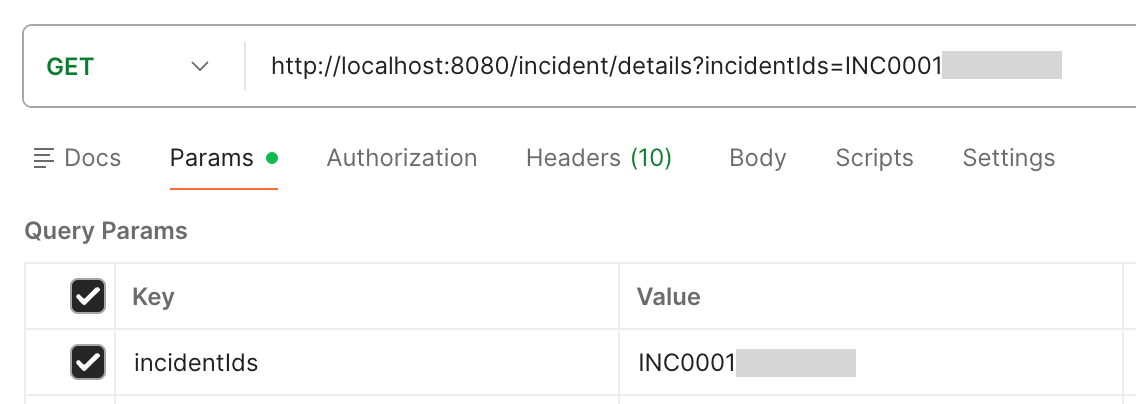
\includegraphics[width=100mm,keepaspectratio]{img/postmanRequest}
		\caption[Exemplo de um Pedido ao Serviço]{Exemplo de um Pedido ao Serviço}
		\label{fig:postmanRequest}
	\end{figure}
	
	Após a execução da análise, o serviço devolve uma resposta, visível na figura \ref{fig:postmanResponse1}, \ref{fig:postmanResponse2} e \ref{fig:postmanResponse3}, contendo a informação principal do incidente, incluindo o seu identificador, título e descrição. A resposta inclui também o resumo gerado pelo \gls{LLM} e uma lista de sugestões de mitigação ordenadas pela prioridade atribuída pelo modelo.
	
	\begin{figure}[H]
		\centering
		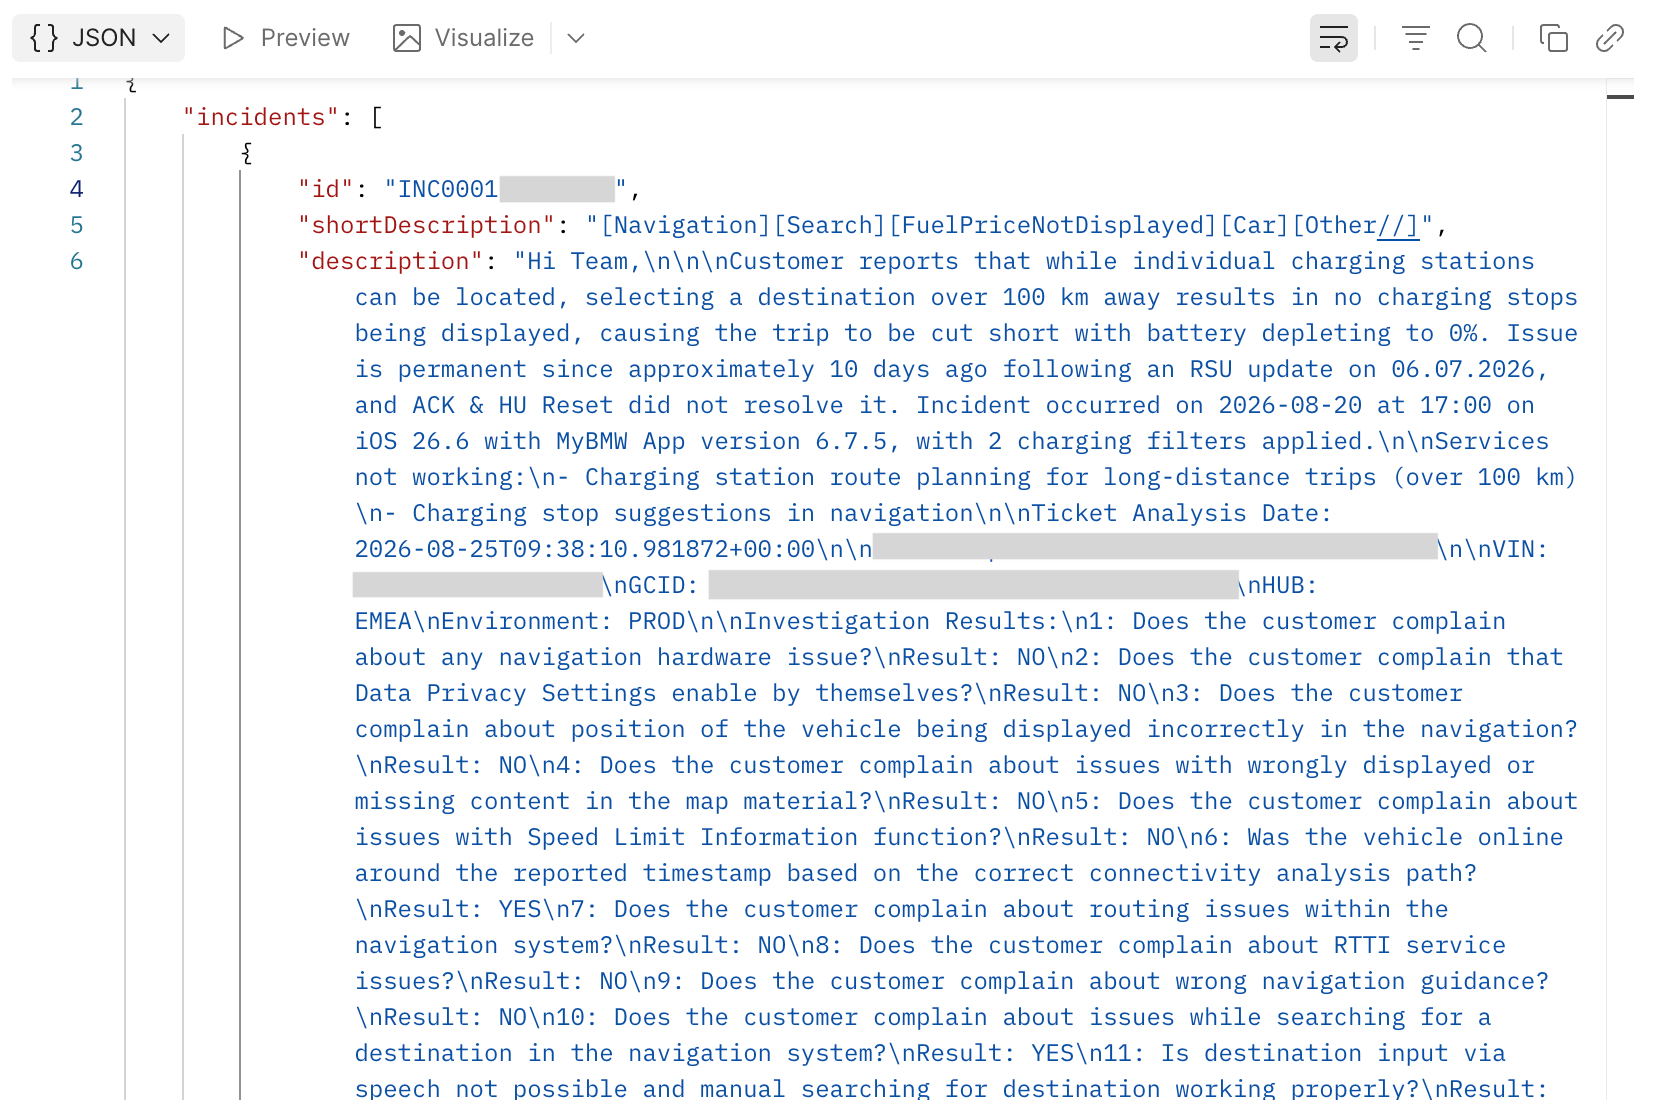
\includegraphics[width=100mm,keepaspectratio]{img/postmanResponse1}
		\caption[Detalhes do Incidente na Resposta do Serviço]{Detalhes do Incidente na Resposta do Serviço}
		\label{fig:postmanResponse1}
	\end{figure}
	
		O exemplo aqui apresentado é uma amostra perfeita de um incidente manual com demasiada informação irrelevante. A descrição deste incidente conta com 2952 letras e 628 palavras, dificultando e atrasando a análise do incidente com informação repetida e irrelevante à investigação e resolução. Já o resumo gerado pelo serviço, descreve o mesmo problema em apenas 399 letras e 71 palavras, indicando uma redução de 88\% de palavras.
	
	\begin{figure}[H]
		\centering
		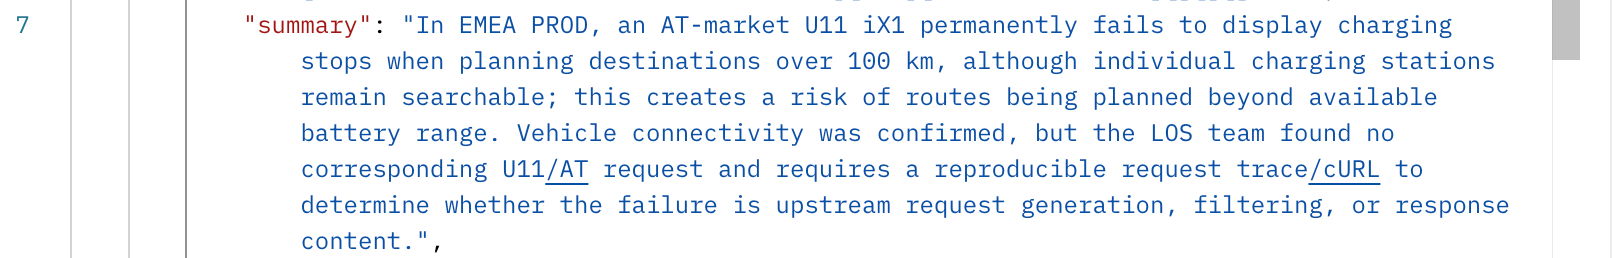
\includegraphics[width=100mm,keepaspectratio]{img/postmanResponse2}
		\caption[Resumo Gerado pelo Serviço]{Resumo Gerado pelo Serviço}
		\label{fig:postmanResponse2}
	\end{figure}
	
	Ainda que o serviço não tenha identificado incidentes relacionados para o contexto do problema, conseguiu, pela própria analise do incidente e com base em documentação relevante, fornecer um resumo e sugestão de investigação correta e passível de ser utilizado pela equipa de suporte.
	
	\begin{figure}[H]
		\centering
		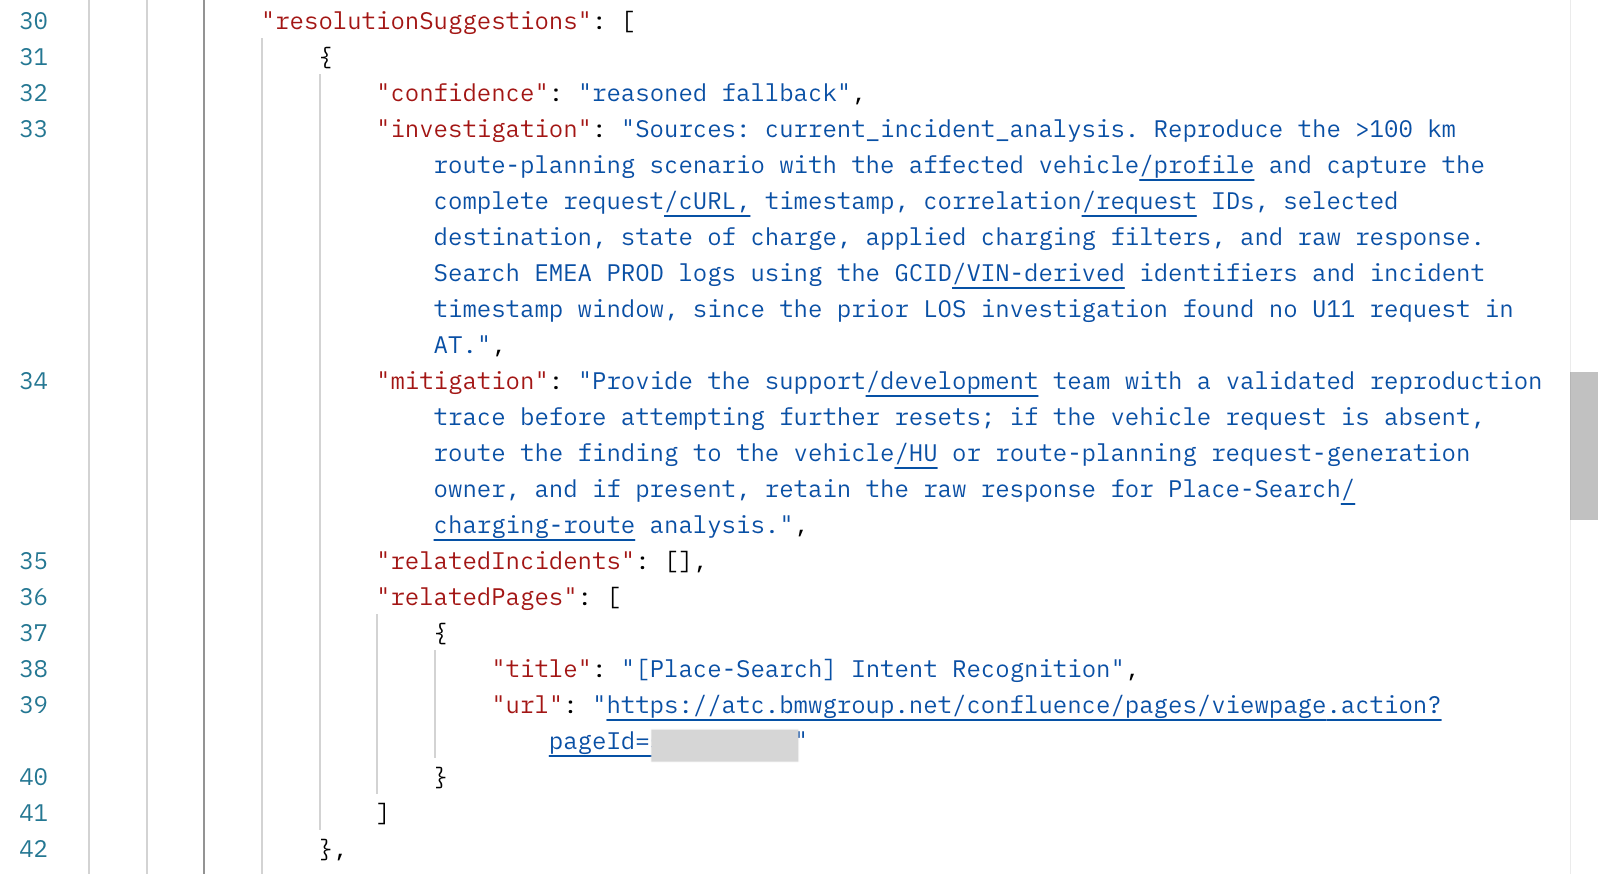
\includegraphics[width=100mm,keepaspectratio]{img/postmanResponse3}
		\caption[Sugestões Geradas pelo Serviço]{Sugestões Geradas pelo Serviço}
		\label{fig:postmanResponse3}
	\end{figure}
	
	Assim sendo, podemos afirmar que cada sugestão contém a informação necessária para compreender e validar a possível solução, incluindo os passos de investigação, a ação de mitigação proposta, os incidentes relacionados e as páginas do \textit{Confluence} consideradas relevantes. Desta forma, a resposta não apresenta apenas uma possível ação para resolver o problema, mas também o contexto utilizado para chegar a essa sugestão.
	
	Por fim, são disponibilizadas informações relativas à execução do \gls{LLM} (figura \ref{fig:postmanResponse5}), nomeadamente o modelo utilizado, o número de \textit{tokens} processados e o custo associado à análise. Estas informações permitem acompanhar o consumo de cada execução.
	
	\begin{figure}[H]
		\centering
		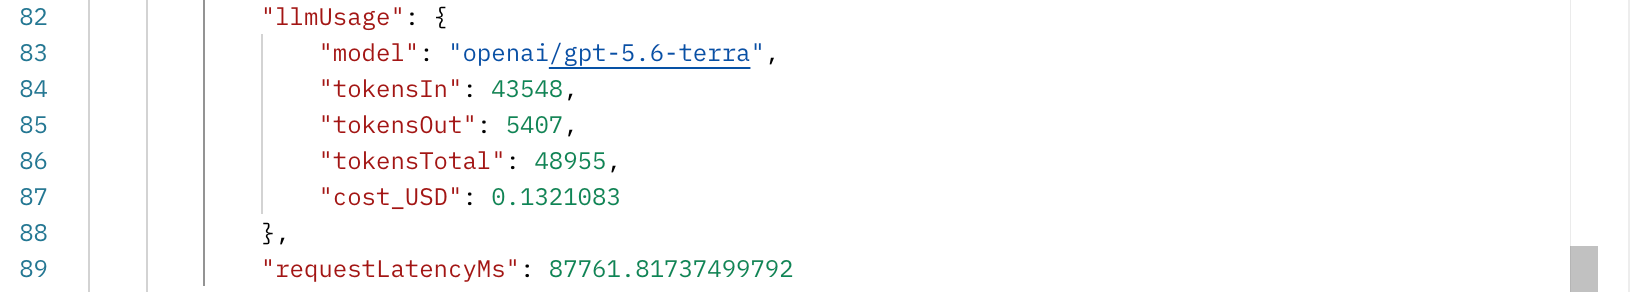
\includegraphics[width=100mm,keepaspectratio]{img/postmanResponse5}
		\caption[Informações Adicionais fornecidas pelo Serviço]{Informações Adicionais fornecidas pelo Serviço}
		\label{fig:postmanResponse5}
	\end{figure}

%----------------------------------------------------------------------------------------
\section{Conclusão}

	Com este capítulo, verificaram-se as principais ferramentas utilizadas, a metodologia aplicada e as decisões implementadas pelo autor do estudo, sendo que estas escolhas tiveram como principal objetivo construir uma solução simples, flexível e adequada ao problema identificado. A implementação permitiu perceber a importância de separar as diferentes responsabilidades da aplicação e de manter as integrações externas isoladas da lógica principal do sistema.
	